\section{Hintergrund}

Die vorliegende Bachelorarbeit hat zum Ziel, die Robotersteuerungssoftware, die
derzeit auf Micro-ROS basiert, auf FreeRTOS zu portieren, um unter anderem einen
vergleichenden Leistungsanalyse zwischen beiden Plattformen durchzuführen. Beide
Systeme sind für die Steuerung eines mobilen Roboters auf einem Cortex-M7
Mikrocontroller von Arm entwickelt, unterscheiden sich jedoch in ihrer
grundlegenden Architektur, was sich auch in ihrer Echtzeitfähigkeit und
Ressourcennutzung widerspiegelt. Während Micro-ROS auf dem \ac{ROS 2} Framework
aufbaut und eine höhere Abstraktionsebene sowie standardisierte
Kommunikationsschnittstellen mittels einer \ac{DDS}-Middleware bietet, basiert
dies selbst auf FreeRTOS. Die Portierung auf FreeRTOS kann daher als eine
Reduzierung der Abhängigkeitsebene betrachtet werden. Dies ermöglicht eine
direktere und effizientere Nutzung der zugrunde liegenden Echtzeit-, sowie
Speicherressourcen.

\begin{figure}[htb] \centering
    \includegraphics[width=0.8\textwidth]{assets/Micro-ROS_architecture}
    \caption{Micro-ROS Architektur\cite[S. 6]{koubaa2023}}
\end{figure}

% Nach der Portierung zu FreeRTOS wird die Echtzeitleistung der Steuerungssoftware
% analysiert mit einem besonderen Fokus auf den Overhead, der durch die
% Micro-ROS-Schicht verursacht wird. Der Vergleich soll aufzeigen, inwiefern
% FreeRTOS durch die Eliminierung dieser zusätzlichen Abhängigkeit eine
% effizientere und leichtgewichtige Lösung für kritische Roboteranwendungen
% darstellt. Dabei soll der Einsatz einer zyklengenaue Messung des Programmablaufs
% ermöglichen, fundierte Aussagen über die Echtzeitfähigkeit beider Plattformen zu
% treffen, und den Leistungsgewinn anhand von diesem Beispiel für eine
% Steuerungssoftware quantitativ zu belegen.

\subsection{FreeRTOS}

FreeRTOS ist ein Open-Source, leichtgewichtiges \ac{RTOS}, das besonders für
eingebettete Systeme geeignet ist. Es zeichnet sich unter anderem durch
deterministisches Verhalten mit Echtzeitgarantie sowie Konfigurierbarkeit von
Heap-Allokationen aus. Diese Eigenschaften machen es zu einer geeigneten Wahl
für mehrfädige Software, insbesondere wenn Echtzeitanforderungen oder fein
abgestimmte Kontrolle über Ressourcennutzung im Vordergrund stehen.

\subsubsection{Features}

FreeRTOS unterscheidet sich von der Bare-Metal-Programmierung dadurch, dass es
einen umfangreichen Abstraktionslayer für den Nutzer bereitstellt. Diese
Abstraktionen ermöglichen es, Echtzeitanforderungen zu bewältigen, ohne dass der
Nutzer diese Funktionalitäten selbst implementieren muss. Beispiele hierfür sind
unter anderem Timer mit konfigurierbarer Genauigkeit (basierend auf den
sogenannten Tick \cite{freertos_rtos_tick, freertos_tick_resolution}), Queues,
Semaphore sowie Mutexe.

Im Fokus dieser Arbeit stehen Queues und auch die sogenannte „Direct Task
Notifications“, die für den Datenaustausch verwendet werden. Ebenfalls relevant
sind Mutexe und „Trace Hooks“ für die anschließende Echtzeitanalyse. Diese
Komponenten werden im Folgenden detailliert erläutert.

\paragraph{Queues}

Queues sind eine Kernkomponente von FreeRTOS. Sie ermöglichen nicht nur
threadsichere Interprozesskommunikation zwischen Tasks, sondern dienen auch
deren Synchronisation. Die bereits vorhandenen
(Ressourcen-)Synchronisationsmechanismen wie Semaphore und Mutexe sind schlicht
auf Queues aufgebaut \cite{freertos_semphr_incl}.

\paragraph{Semaphore und Mutexe} \label{sec:mutex}

Wie bereits erwähnt, sind Semaphore und Mutexe Mechanismen zur Koordinierung des
Zugriffs auf gemeinsame Ressourcen. Aufgrund ihrer Einfachheit eignen sich
Semaphore zusätzlich für die Task-Synchronisation. Semaphoren sind somit
Synchronisationsmechanismen ohne Prioritätsvererbung -- ein Konzept, bei dem
eine niedriger priorisierte Task, die einen \textit{Mutex} hält, temporär auf
die Priorität der wartenden Task angehoben
wird~\cite{wikipedia_priority_inheritance}. Diese Funktionalität fehlt bei
Semaphoren, wodurch es zur Prioritätsinversion kommen kann: Eine höher
priorisierte Task wird blockiert, während der Scheduler stattdessen eine
niedriger priorisierte Task ausführt, bis die benötigte Ressource freigegeben
ist. \cite{wikipedia_priority_inversion}.

Die folgenden Grafiken veranschaulichen ein Beispiel jeweils für
Prioritätsinversion und Prioritätsvererbung:

\begin{figure}[H]
    \centering
    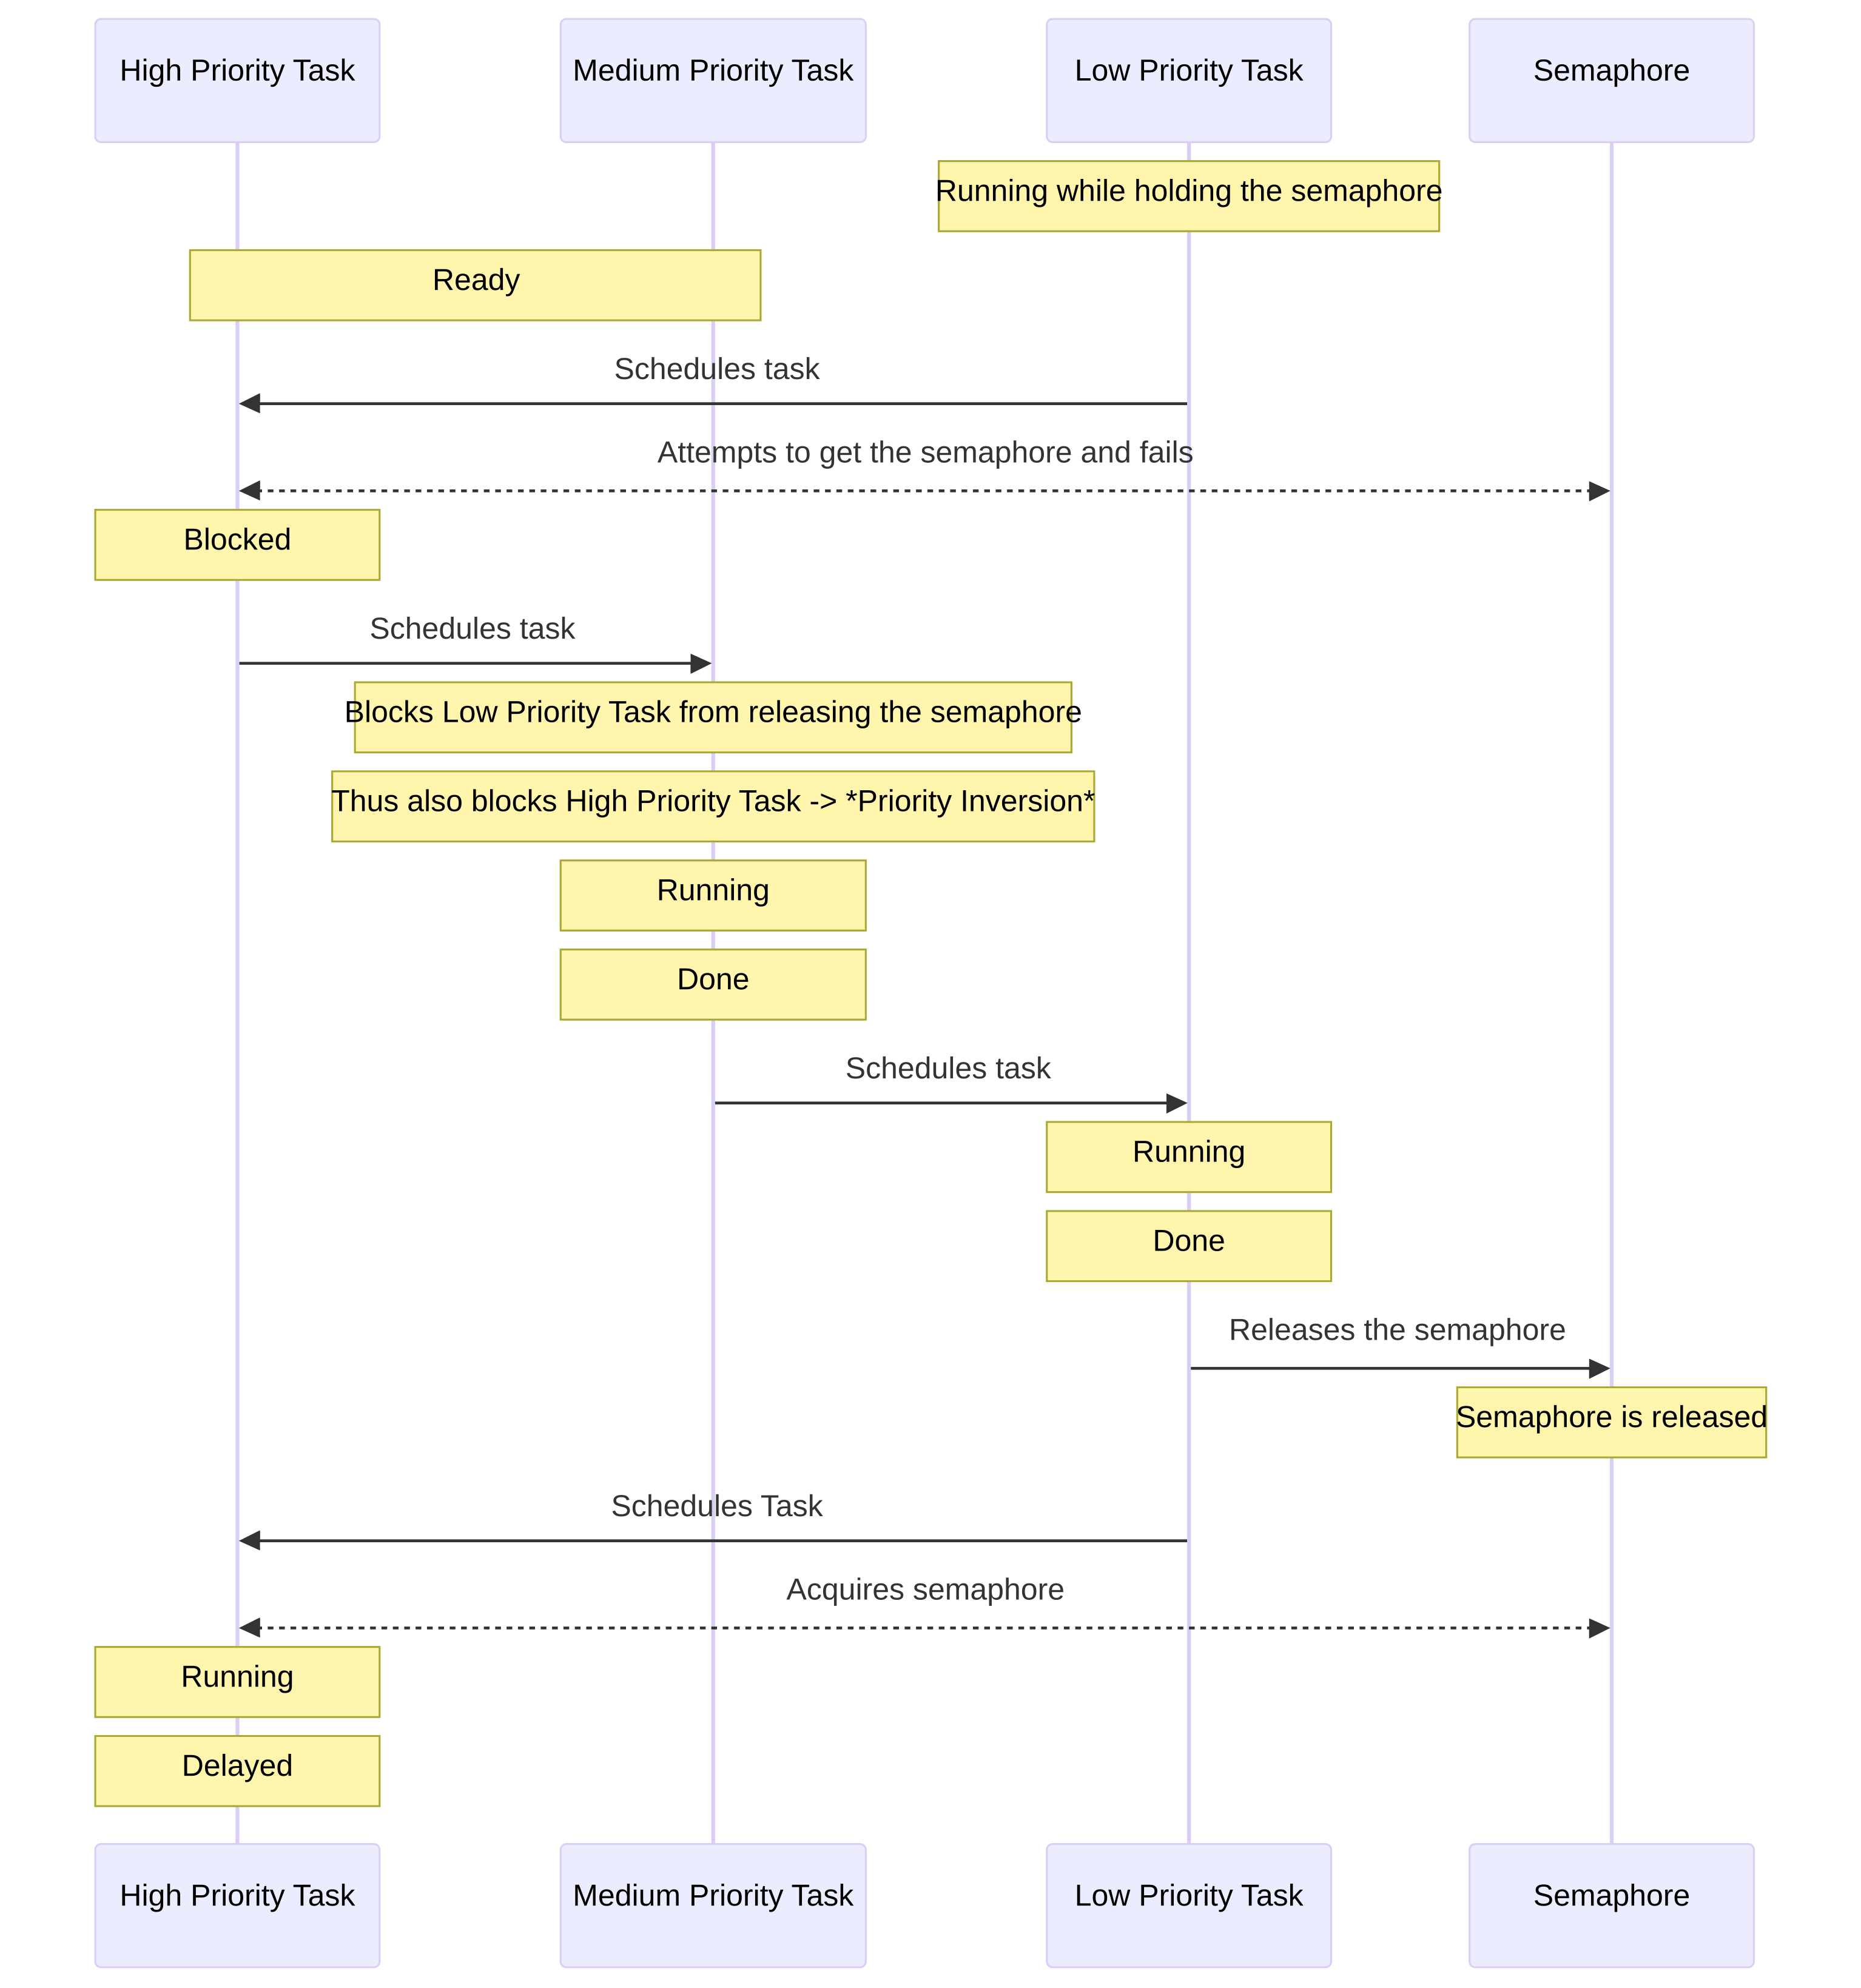
\includegraphics[width=1\textwidth]{assets/prio_inversion}
    \caption{Prioritätsinversion}
\end{figure}

\begin{figure}[H]
    \centering
    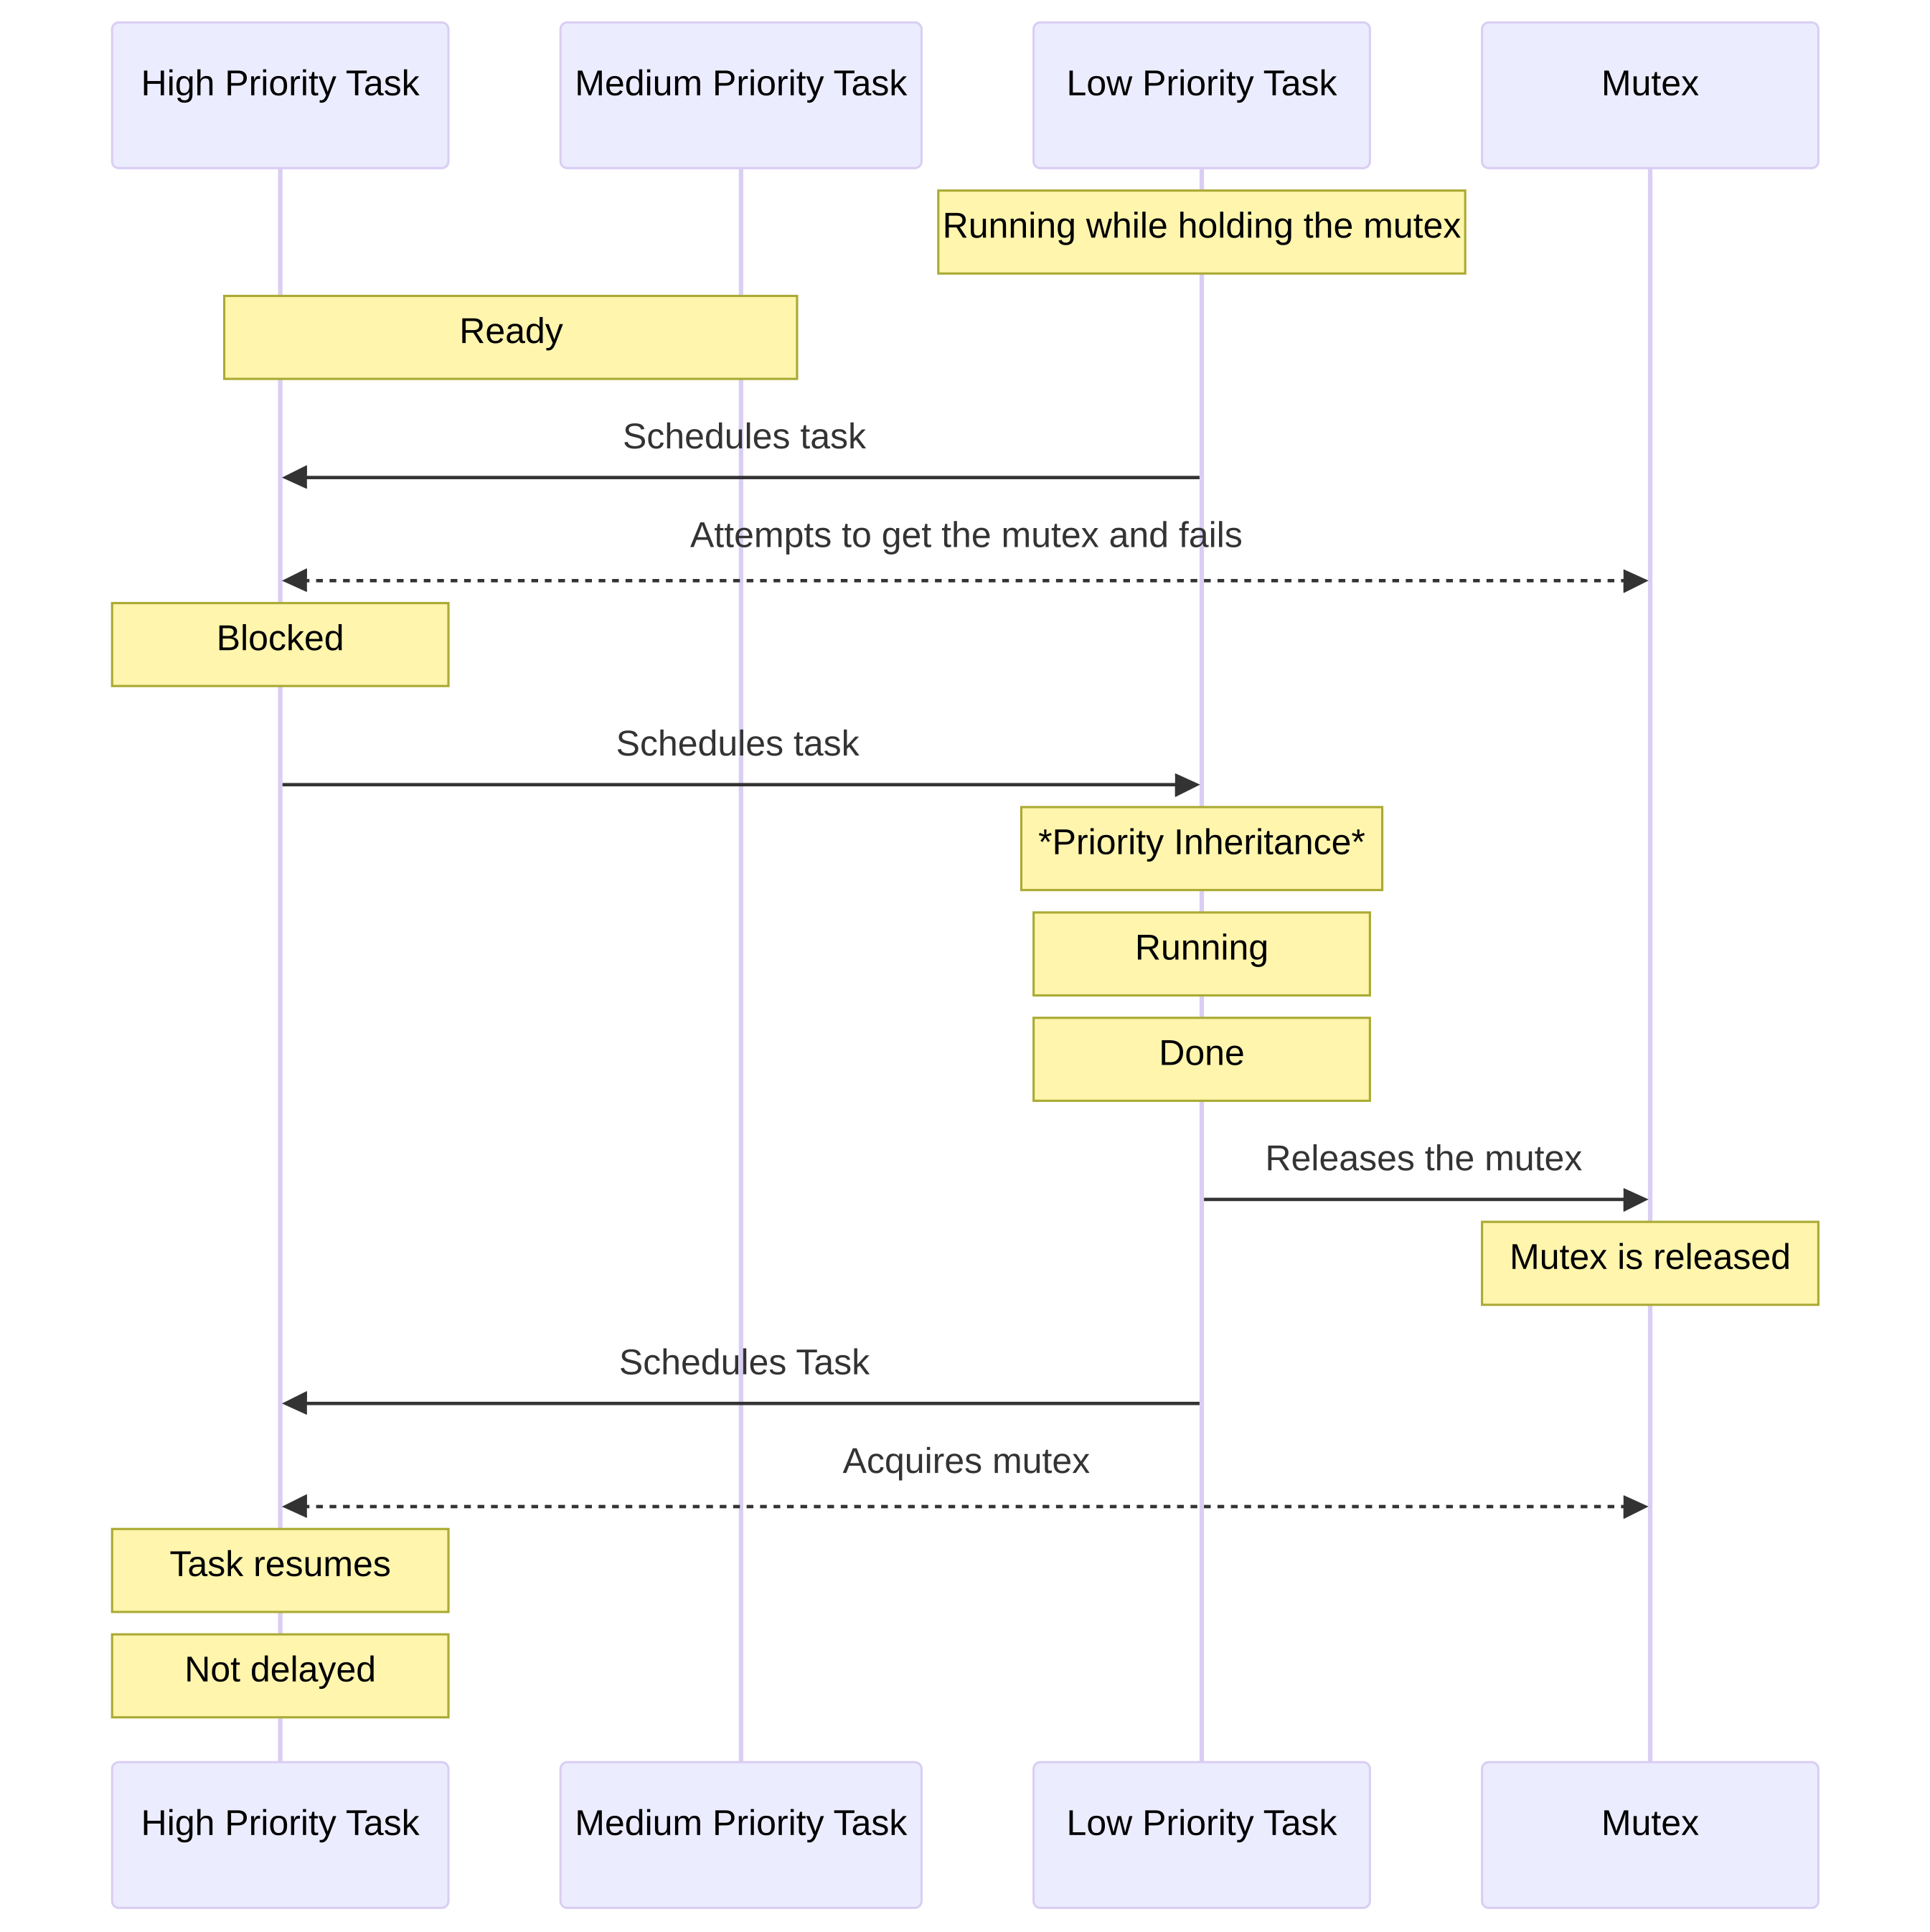
\includegraphics[width=1\textwidth]{assets/prio_inheritance}
    \caption{Prioritätsvererbung}
\end{figure}

\paragraph{Direct Task Notifications} \label{sec:direct_task_notification}

Direct Task Notifications sind ein effizienterer und ressourcenschonenderer
Mechanismus zur Task-Synchronisation \cite{freertos_task_notifications_desc}.
Insbesondere soll das Entblocken einer Task mittels Direct Task Notifications
bis zu 45\% schneller sein und weniger RAM benötigen
\cite{freertos_task_notifications_usage}. Im Gegensatz zu Semaphoren, die als
separate Objekte fungieren, kommunizieren sie direkt mit Tasks durch
Modifikation eines internen Task-Zählers \cite{freertos_tasks_c_308}. Analog zur
Handhabung von Semaphoren wird mittels Funktionen wie
\mintinline{c}|xTaskNotifyGive()| dieser Zähler
inkrementiert~\cite{freertos_tasks_c_4990}, während
\mintinline{c}|ulTaskNotifyTake()| ihn wieder
dekrementiert~\cite{freertos_tasks_c_4614}. 

\paragraph{Trace Hooks} \label{sec:trace_hooks}

„Trace Hooks“ sind spezielle, von FreeRTOS bereitgestellte Makros. Sie
ermöglichen beispielsweise die Verfolgung oder Protokollierung von
Systemereignissen. Diese Makros werden innerhalb von Interrupts beim Scheduling
aufgerufen und sollten stets vor der Einbindung von
\mintinline{text}|FreeRTOS.h| definiert werden \cite{freertos_rtos_trace_hooks}.

\subsection{Nutzung von Caches}

Caches sind schnelle Speicherkomponenten, die dazu dienen, Zugriffe auf häufig
verwendete Daten und Befehle zu beschleunigen und den Energieverbrauch zu
reduzieren \cite{ka001150}. In vielen modernen Mikrocontrollern, wie dem
Cortex-M7, ist der L1-Cache (Level 1 Cache) jeweils in einen Datencache
(D-Cache) sowie einen Instruktionscache (I-Cache) unterteilt \cite[S.
6]{an4667}. Da Zugriffe auf den Hauptspeicher und Flash-Speicher generell
deutlich langsamer sind und mehrere Taktzyklen
benötigen~\cite{stm32_memory_sections}, ermöglichen L1-Caches
Zero-Wait-State-Zugriffe~\cite[S. 6]{an4667}. Dadurch kann der Prozessor ohne
zusätzliche Wartezyklen auf Daten zugreifen \cite{waitstate_wiki}.

% TODO: everything AHB connect to AXI
Der L1-Cache kann nur mit Speicherschnittstellen auf der \ac{AXI}-Busarchitektur
genutzt werden~\cite[S. 4]{an4839}. Hierzu zählen unter anderem der Flash, der
\ac{SRAM} sowie die beiden \ac{AHB}-Busse, die alle an den AXI-Bus angebunden
sind (\ref{fig:m7_sys_arch}).

\begin{figure}[htb]
    \centering
    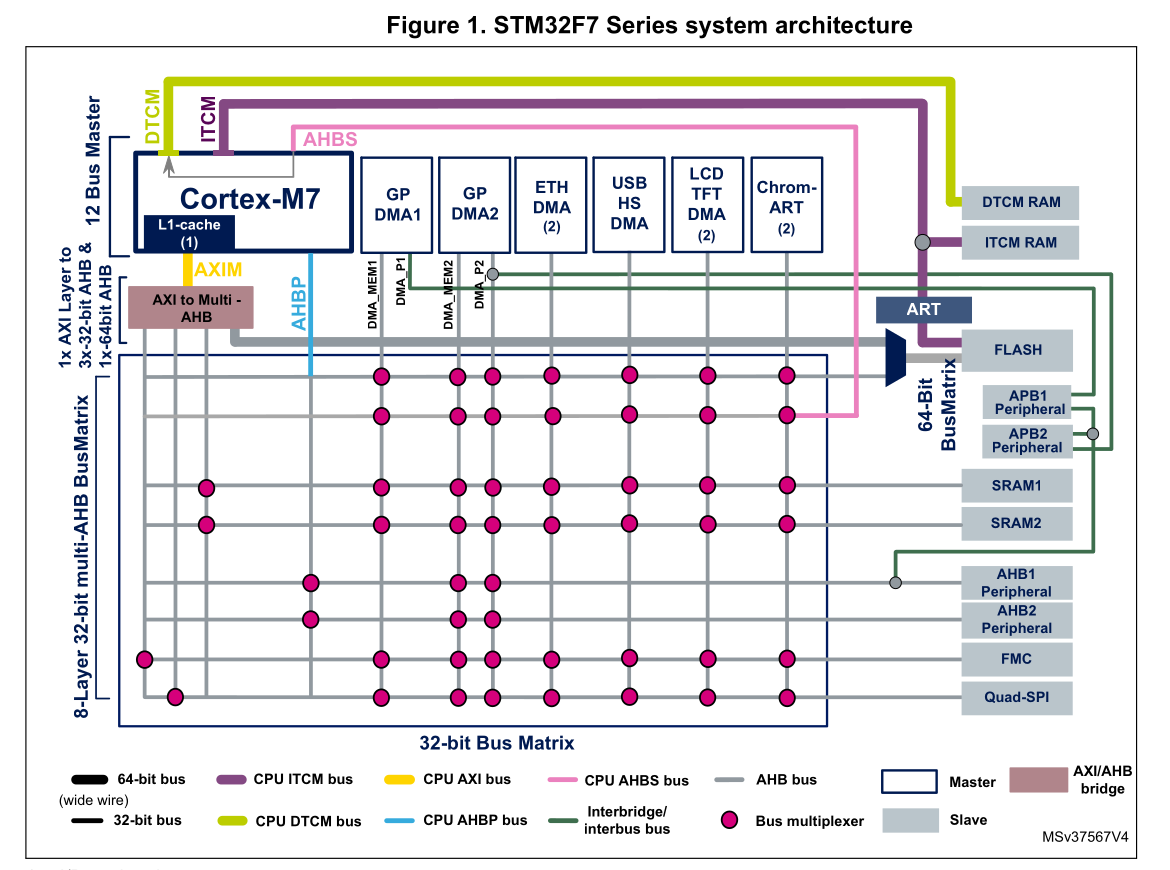
\includegraphics[width=1\textwidth]{assets/m7_system_arch}
    \caption{STM32F7 Systemarchitektur \cite[S. 9]{an4667}}
    \label{fig:m7_sys_arch}
\end{figure}

Aus der Matrix wird deutlich, dass für den Speicher zwischen SRAM und TCM-RAM
unterschieden wird. Der \ac{TCM} verfügt jeweils für Instruktionen und Daten
über einen dedizierten Kanal zum Prozessor und ist nicht cachefähig, bietet aber
als Besonderheit niedrigere Zugriffszeiten als SRAM. Während bei SRAM die
Zugriffszeit variieren kann (schnell aus dem Cache oder langsam aus dem
Speicher), ist die Zugriffszeit bei TCM konsistent und deterministisch.
Dies macht sie besonders geeignet für zeitkritische Routinen wie Interrupt-Handler
oder Echtzeitaufgaben. (\cite{arm_den0042}) % TODO TCM wird nicht in der arbeit betrachtet

Zusammenfassend lässt sich sagen, dass jeder normale, nicht gemeinsam genutzte
(non-shared) Speicherbereich gecacht werden kann, sofern er über das AXI-Bus
zugänglich ist \cite[S. 4]{an4839}~\cite[S. 7]{an4667}.

Aus der Tabelle für den internen Speicher wird deutlich, dass der Flash ab der
Adresse $0x0800 0000$ über das AXI-Bus angesprochen wird
(\ref{fig:internal_mem_table}). Diese Adresse ist auch im Linker-Skript
standardmäßig für den Flash festgelegt. Daher kann der I-Cache über den AXI-Bus
für den Flash genutzt werden, sofern der Boot-Pin sowie die assoziierten
\mintinline{text}|BOOT_ADDx| Option unverändert bleiben und die Firmware an die
Standardadresse geflasht wird \cite[S. 28]{stm32_datasheet}.

\begin{figure}[htb]
    \centering
    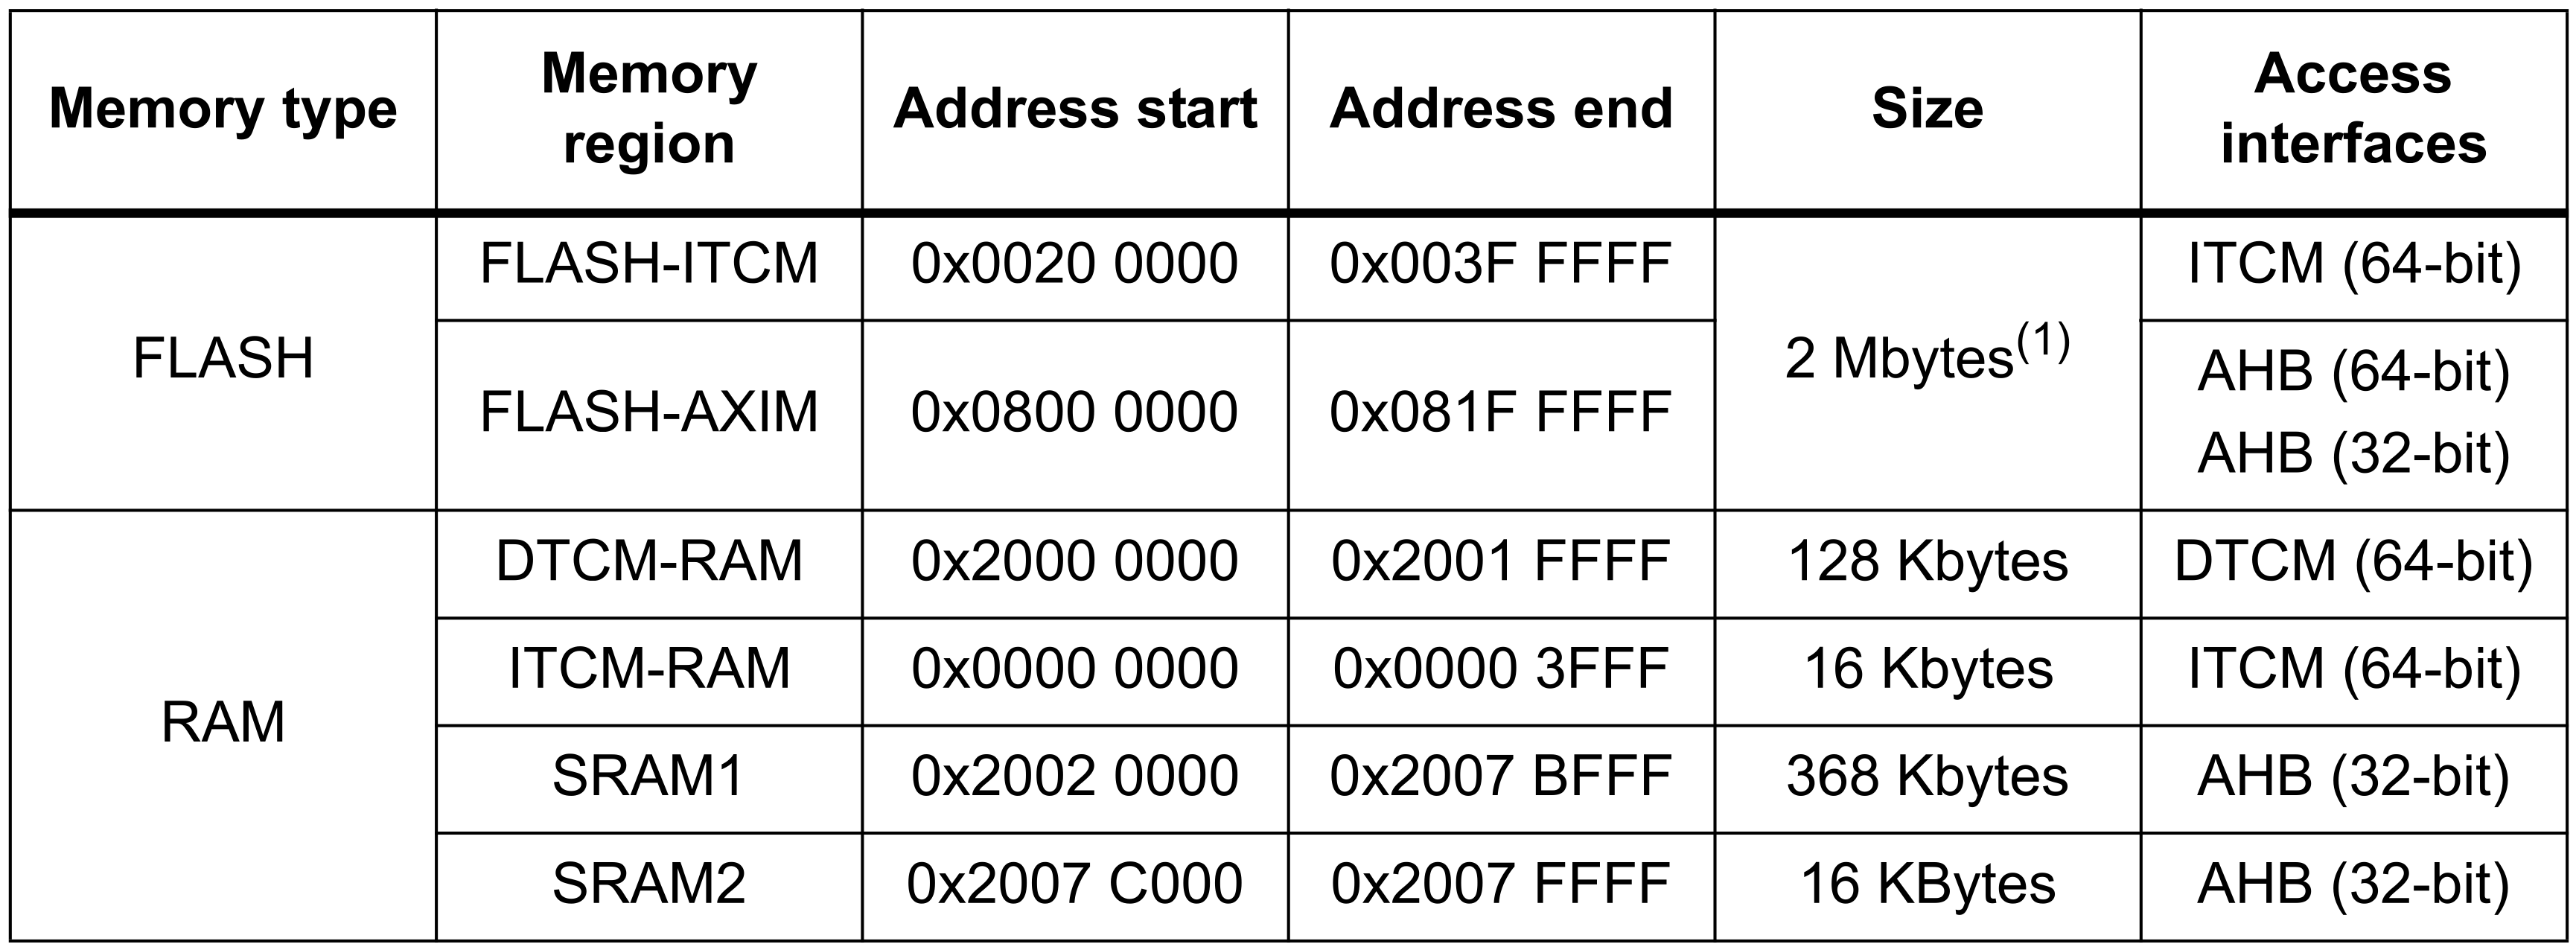
\includegraphics[width=1\textwidth]{assets/internal_mem_table}
    \caption{STM32F7 Speicheradressen \cite[S. 14]{an4667}}
    \label{fig:internal_mem_table}
\end{figure}

\begin{code}
\begin{minted}{c}
MEMORY
{
RAM (xrw)      : ORIGIN = 0x20000000, LENGTH = 512K
FLASH (rx)      : ORIGIN = 0x8000000, LENGTH = 2048K
}
\end{minted}
    \captionof{listing}{Definition Speicherbereich im Linker-Script für STM32F7}
\end{code}

Um Caches zu nutzen, bietet die STM-\ac{HAL} dedizierte Funktionsaufrufe in der
API an \cite[S. 4]{an4839}:

\begin{code}
\begin{minted}{c}
void SCB_EnableICache(void)
void SCB_EnableDCache(void)
void SCB_DisableICache(void)
void SCB_DisableDCache(void)
void SCB_InvalidateICache(void)
void SCB_InvalidateDCache(void)
void SCB_CleanDCache(void)
void SCB_CleanInvalidateDCache(void)
\end{minted}
    \captionof{listing}{Cache-Funktionen}
\end{code}

Bei einer Cache-Clean werden modifizierte Cache-Zeilen (Dirty Cache Lines), die
durch das Programm aktualisiert wurden, zurück in den Hauptspeicher geschrieben
\cite[S. 4]{an4839}. Dieser Vorgang wird gelegentlich auch als „flush”
bezeichnet. Eine Cache-Invalidierung markiert den Inhalt des Caches als
ungültig, sodass bei einem erneuten Zugriff auf dieselben Daten der Speicher neu
ausgelesen und der Cache aktualisiert werden muss.

Allerdings kann beim Aktivieren von Caches für Speicherbereiche, die vom
DMA-Controller genutzt werden, ein Problem der Cache-Kohärenz (Cache Coherency)
entstehen, da der Prozessor in diesem Fall nicht mehr der einzige Master ist,
der auf diese Speicherbereiche zugreift.

\subsubsection{Cache-Clean bei DMA} \label{sec:cache_clean}

Damit der DMA-Controller stets auf korrekte Daten zugreifen kann, ist eine
Cache-Clean nach jeder Modifikation der Daten erforderlich \cite[S. 6]{an4839}.
Ohne diesen Schritt würden die Änderungen nicht im SRAM widergespiegelt, und der
DMA-Controller würde weiterhin veraltete Daten verwenden.

\subsubsection{Cache-Invalidierung bei DMA}

Bei Daten, die aus dem Speicher gelesen werden, auf die auch der DMA-Controller
zugreift und modifiziert, muss vor jedem Lesevorgang eine Cache-Invalidierung
erfolgen \cite{embeddedexpert_cache}. Da der DMA-Controller die Daten jederzeit
ändern kann, sind die gecachten Daten per se ungültig und müssen immer durch
Aktualisierung ersetzt werden.

\subsection{Methode zur Echtzeitanalyse} \label{sec:dwt}

Um die Echtzeitanalyse der Steuerungssoftware durchzuführen, ist eine Methode
erforderlich, mit der beliebige Ausführungsabschnitte der Software flexibel,
präzise und threadsicher gemessen werden können. Da die Software multithreaded
ist, muss ebenfalls sichergestellt werden, dass die Messungen trotz preemptivem
Scheduling sowie Interrupts korrekt und zyklengetreu durchgeführt werden können.

Basierend auf den oben genannten Herausforderungen bietet die \ac{DWT} als eine
geeignete Lösung \cite{ARM_KA001499}. Die DWT ist ein Debug-Einheit in
Prozessoren inklusive ARMv7-M \cite{ARMv7_ref_man_dwt_about}, die das Profiling
mittels verschiedener Zähler unterstützen \cite{ARMv7_ref_man_dwt_profiling}.
Ein für diese Arbeit zentraler Teil der DWT ist der Zyklenzähler
\mintinline{c}|DWT_CYCCNT|, der bei jedem Takt inkrementiert wird, solange sich
der Prozessor nicht im Debug-Zustand befindet \cite{ARMv7_ref_man_dwt_cycle}.
Dadurch ermöglicht die DWT beispielsweise die Erfassung von Echtzeitaspekten mit
zyklengenauer Präzision under normaler Operation \cite{ARMv7_ref_man_dwt}.

\subsubsection{Beispiel: Segger SystemView}

Ein Beispiel hierfür ist Segger SystemView, ein Echtzeit-Analysewerkzeug, das
die DWT einsetzt, um Live-Code-Profiling auf eingebetteten Systemen
durchzuführen \cite{SEGGER_SystemView}.

Das Segger SystemView nutzt den DWT-Zyklenzähler, indem die Funktion \linebreak
\mintinline{c}|SEGGER_SYSVIEW_GET_TIMESTAMP()| für Cortex-M3/4/7-Prozessoren
einfach die hardkodierte Registeradresse des Zyklenzählers zurückgibt \cite[S.
65]{Segger_SystemView_manual}\cite{Arm_DWT_Programmers_Model}, anstatt die
interne Funktion \mintinline{c}|SEGGER_SYSVIEW_X_GetTimestamp()| aufzurufen.
